
\chapter{面向海上雾天场景的小目标检测模型设计}
\label{chap:method}

本章以实时端到端检测器RT-DETR为基准框架，围绕海上雾天航拍小目标检测中普遍存在的特征弱化、语义混淆与端侧实时约束，对检测网络的主干结构与雾天鲁棒性机制进行优化设计，首先通过改进轻量化主干网络并引入多维注意力机制，提升微小目标特征的底层表达能力。其次构建基于状态空间模型的雾分布表征分支，以实现雾天细节信息与环境先验的有效提取。随后设计动态物理引导特征融合机制，加强环境先验与深层语义信息的协同表达。最后提出分阶段协同训练策略，以保障模型在复杂环境下的稳定收敛与整体检测性能，构建兼顾实时性与鲁棒性的轻量级检测模型。


\section{端到端雾天目标检测算法整体框架}
\label{sec:overall_framework}


本文在实时目标检测模型 RT-DETR 的基础上构建了包含检测主干与物理先验辅助分支的协同结构，在特征层面引入了物理先验注入与语义融合。整体架构如图\ref{fig:overall_arch}所示。

\begin{figure}[!htbp]
    \centering
    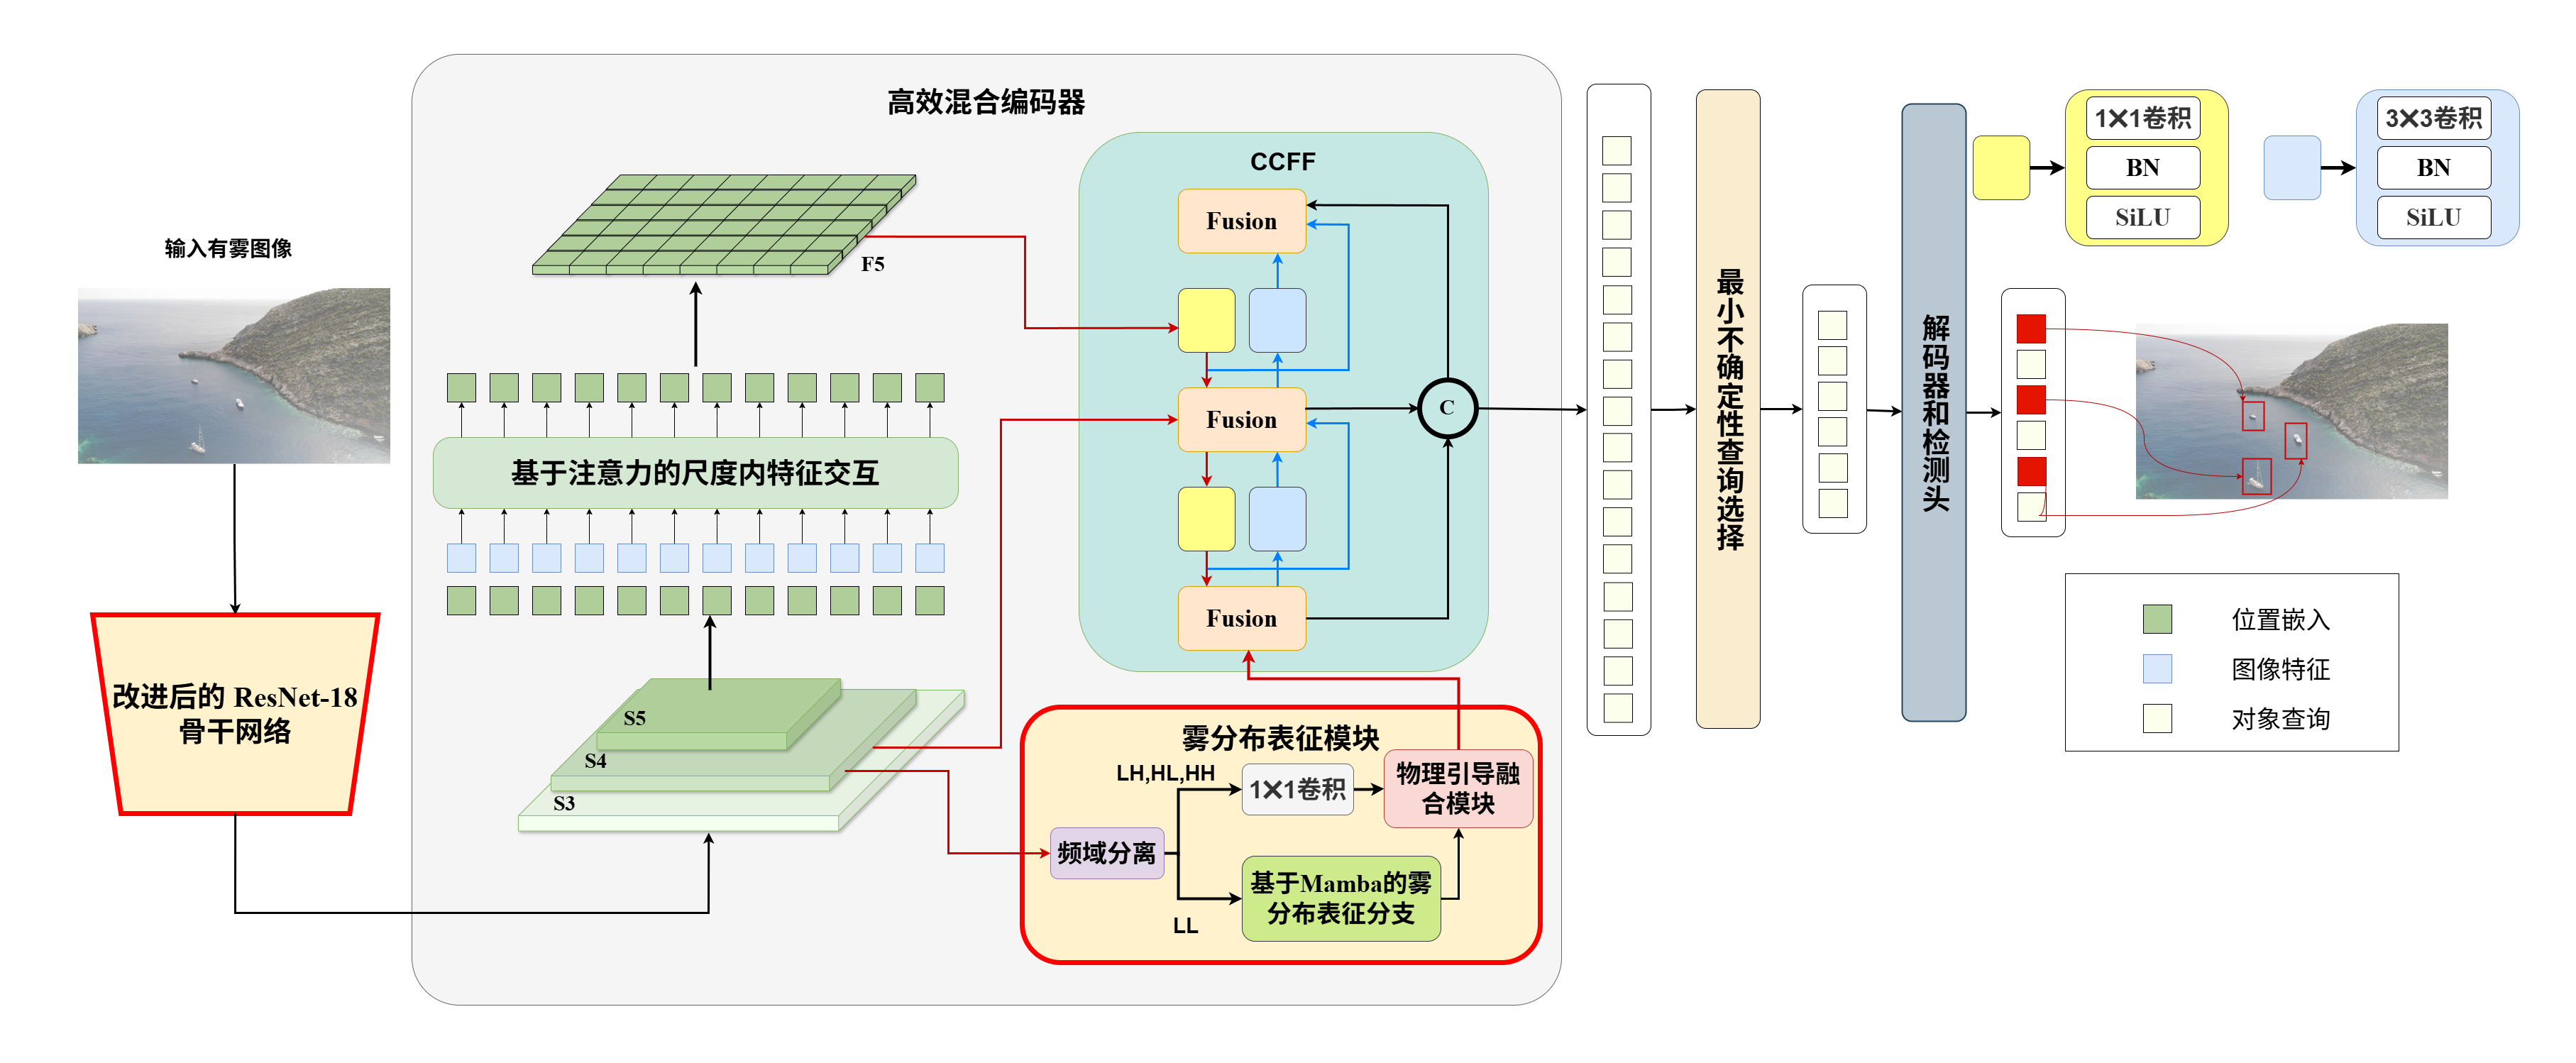
\includegraphics[width=1.0\linewidth]{figures/模型整体架构图.png}
    \caption{面向海上雾天场景的小目标检测总体架构示意}
    \label{fig:overall_arch}
\end{figure}

网络主要由轻量化检测主干、加入雾分布表征模块的混合编码器以及解码器和检测头共同组成。针对微小目标特征弱化与常规主干网络计算资源消耗过大的问题，本文设计基于多维注意力机制的轻量级主干网络，将三维无参数注意力与倒残差自注意力引入特征提取阶段以增强微弱目标的底层语义表达能力。为解决常规网络将去雾与检测作为串行孤立任务导致的特征冲突问题，本文构建基于频域解耦与状态空间模型的雾分布表征分支，并设计动态物理引导特征融合机制，将雾分布作为物理先验自适应注入检测特征流，实现环境先验与语义信息的协同表达。

从算法的整体数据流向来看，输入雾天图像$I_{fog}$首先进入检测主干，由轻量化残差网络逐层降维提取多尺度语义特征。在主干的特定中间特征层，网络分流构建雾分布表征分支，该分支并不以生成视觉上绝对清晰的图像为终极目标，而是以提取雾气空间分布物理表征为核心任务，为后续特征的选择性增强提供依据。提取的物理先验与主干语义特征在颈部节点交汇，经动态融合模块后，送入高效混合编码器完成尺度内特征交互与跨尺度融合，最终由端到端解码器输出目标类别与边界框。在模型优化的训练策略层面，为保证雾分布表征具有物理意义并被检测网络有效利用，本文采用分阶段协同训练流程。训练阶段首先对雾分布表征分支进行独立预训练，使其在清晰监督下形成稳定表征，避免联合训练初期因检测损失主导而产生无意义响应，随后进入联合微调阶段。为解决联合模型训练初期梯度震荡以及端到端一对一匹配导致的正样本不足问题，在检测微调阶段引入协作混合分配方案，通过并行辅助预测头提供更密集的监督信号。在最终的推理部署阶段，辅助检测头与重构监督支路被完全移除，仅保留主解码器的集合预测输出，从而在不增加任何额外推理计算成本的前提下，有效保障了联合模型的稳定收敛并大幅提升了雾天微小目标的检测召回率。
接下来将详细阐述每个模块的设计思路和实现细节。

\section{基于多维注意力机制的轻量化主干网络设计}
\label{sec:backbone}

海上无人机平台通常受限于机载算力、功耗与内存带宽等约束，检测模型在部署时需要在精度与实时性之间取得平衡。本文选用 RT-DETR 作为基准检测框架，该框架结合了 CNN 的局部特征提取能力与 Transformer 的全局建模能力，并通过轻量化编码器与 IoU-aware 优化策略实现了高效的端到端集合预测（其基础架构如图3-6所示）。RT-DETR由一个主干网络、一个高效混合编码器和一个带有辅助预测头的Transformer解码器组成。它将主干网络最后三个阶段的特征{S3,S4,S5}输入到编码器中。高效混合编码器通过尺度内特征交互(AIFI)和跨尺度特征融合(CCFF),将多尺度特征转换为一系列图像特征。随后,采用不确定性最小查询选择方法(IoU),选择固定数量的编码器特征作为解码器的初始对象查询。最后,带有辅助预测头的解码器迭代优化对象查询,以生成类别和边框。

\begin{figure}[!htbp]
    \centering
    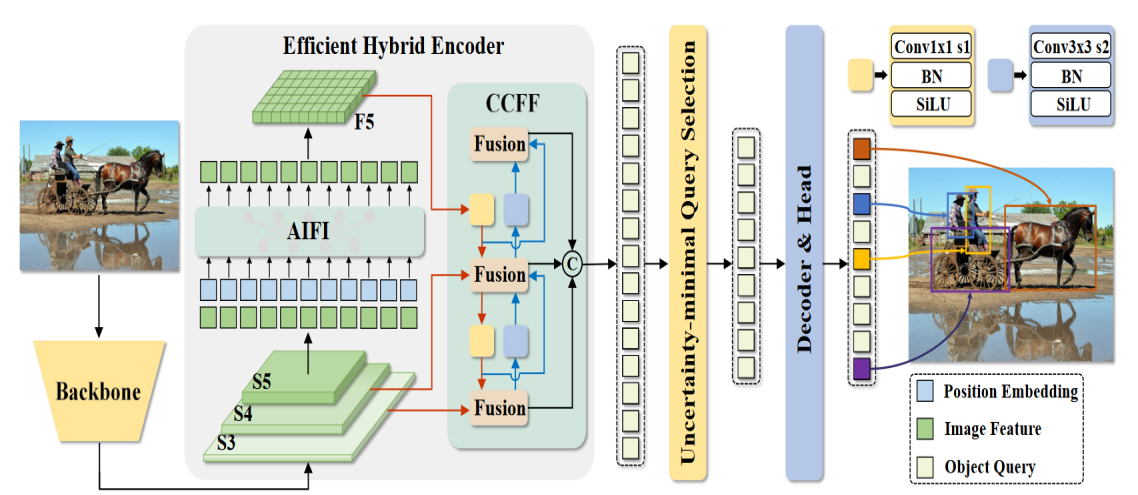
\includegraphics[width=0.9\linewidth]{figures/RT-DETR模型架构图.png}
    \caption{RT-DETR模型架构图}\label{Fig2-3}
\end{figure}


然而，原始架构在处理雾天海面微小目标时，由于特征空间分布极不均匀，目标边缘与局部纹理往往在深层网络中发生不可逆的退化。为此，本文提出一种适用于有雾天气航拍小目标检测的改进主干网络（架构如图3-7所示）。在语义特征提取阶段，本文选用参数规模更小的 ResNet-18 替代原始深层骨干，以显著降低前向推理延迟。ResNet-18 是一个较浅的网络，其参数量和计算量远小于 RT-DETR 中使用的 ResNet-50 。这使得它在推理时的速度更快，更适合对实时性要求高的任务。并且通常无人机搭载的计算单元在资源有限的设备上，ResNet-18由于计算量小，能够更好地适应这些资源受限的环境。虽然ResNet-18层数较少，但是在小目标检测任务中有时并不需要极其深层的特征提取网络。ResNet-18能够提供足够的特征抽象层级来满足此类任务的需求，在较小规模数据集上训练时也不容易过拟合。为弥补网络深度缩减带来的特征抽象能力下降，本文在残差模块中创新性地集成了无参数三维能量注意力机制（SimAM）与倒残差多头自注意力模块（iRMB）。前者基于神经科学统计理论抑制海面动态噪声并放大微弱高频特征；后者则在低计算复杂度下实现长距离全局交互，从而在维持轻量化的同时极大提升了网络对雾天小目标的特征保真与语义判别能力。

\begin{figure}[!htbp]
    \centering
    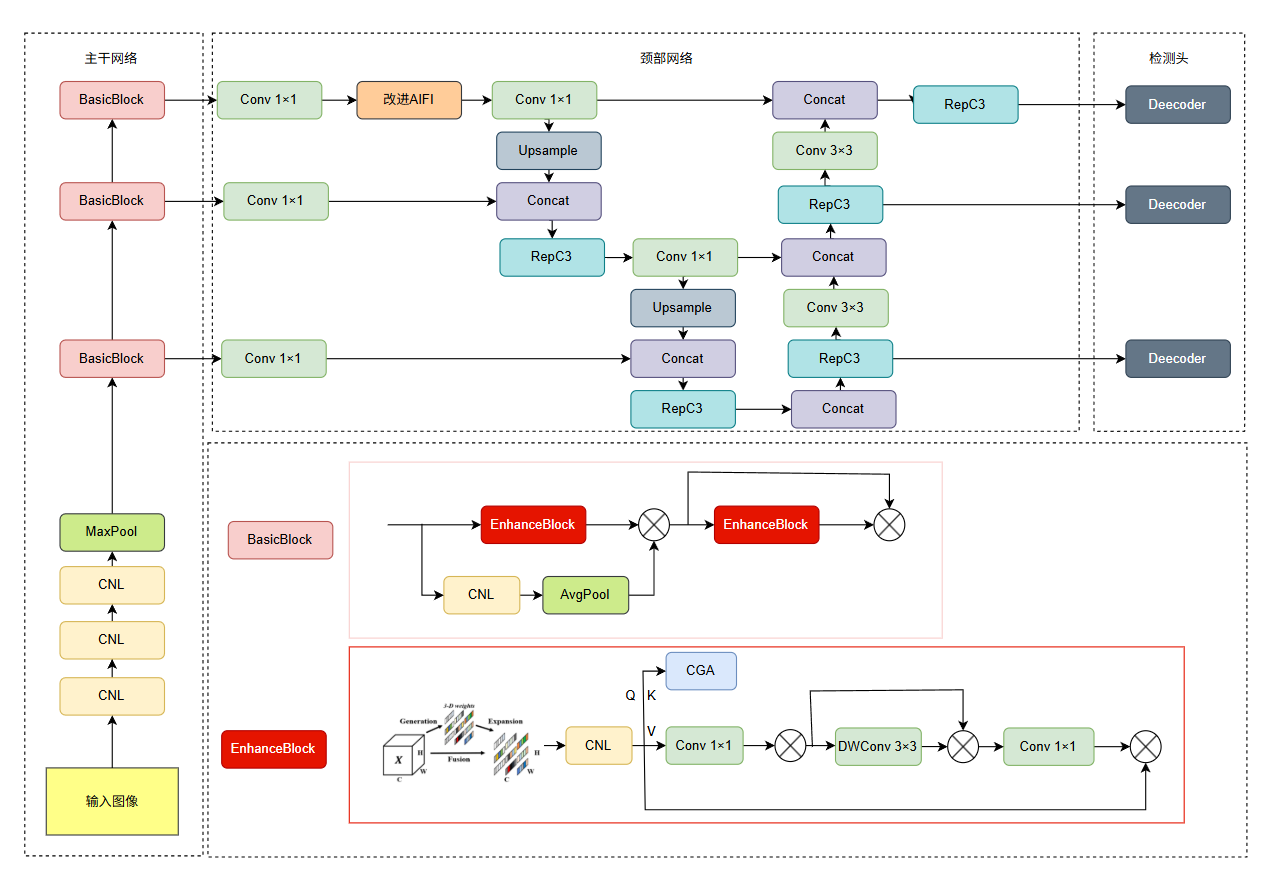
\includegraphics[width=0.9\linewidth]{figures/改进RTDETR模型架构图.png}
    \caption{改进RTDETR模型架构图}\label{Fig2-3}
\end{figure}

\subsection{无参数三维注意力模块}

为增强主干网络对微弱目标结构的选择性响应，本文在残差基本块内部引入无参数三维注意力模块（SimAM）。该模块为每个神经元定义了一个能量函数，有效地帮助模型学习小目标的特征，抑制非目标背景干扰，增强特征映射的表示能力，从而提高模型检测精度，弥补了RT-DETR算法在小目标处理上的不足。其结构如下图所示。

\begin{figure}[!htbp]
    \centering
    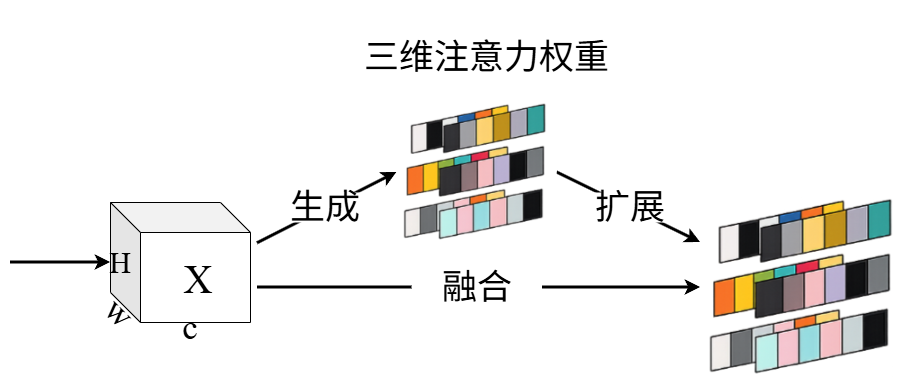
\includegraphics[width=0.8\linewidth]{figures/SimAM结构图.png}
    \caption{三维注意力模块}\label{Fig2-3}
\end{figure}


无参数三维注意力模块是一个轻量级的注意模块，可以自适应地调整特征图中不同位置的重要性，并通过计算相似度得分和加权特征来提高目标检测的准确性。为了更好地实现注意力，找到重要神经元最简单的方法是测量神经元之间的线性可分性。在该模块中定义的能量函数，如式 \eqref{eq:simam_energy_3} 所示。无参数三维注意机制模块不需要在原始网络中添加参数，而是在一层中推断出特征图的三维注意权值。
设输入特征为单通道特征图 $X\in\mathbb{R}^{H\times W}$，其中目标神经元记为 $t$，其余神经元记为 $\{x_i\}_{i=1}^{M-1}$，$M=H\times W$ 表示该通道神经元总数。引入线性变换 $\hat{t}=w_t t+b_t$ 与 $\hat{x}_i=w_t x_i+b_t$，并构造如下能量函数：
\begin{equation}
e_t(w_t,b_t,y,x_i)=\bigl(y_t-\hat{t}\bigr)^2+\frac{1}{M-1}\sum_{i=1}^{M-1}\bigl(y_o-\hat{x}_i\bigr)^2 ,
\label{eq:simam_energy_3}
\end{equation}
式中，$y_t$ 与 $y_o$ 分别表示目标神经元与其余神经元的二值监督信号（在推导中取 $y_t=1$、$y_o=-1$），$w_t$ 与 $b_t$ 为线性变换的权重与偏差。最小化式 \eqref{eq:simam_energy_3} 等价于训练同一通道内神经元 $t$ 与其余神经元之间的线性可分性。由于同一通道内神经元可近似服从相同分布，均值与方差可预先计算以避免冗余运算，能量函数可进一步写为
\begin{equation}
e_t(w_t,b_t,y,x_i)=\frac{1}{M-1}\sum_{i=1}^{M-1}\bigl(-1-(w_t x_i+b_t)\bigr)^2+\bigl(1-(w_t t+b_t)\bigr)^2+\lambda w_t^2 ,
\label{eq:simam_energy_4}
\end{equation}
其中 $\lambda$ 为正则化系数。对式 \eqref{eq:simam_energy_4} 求解可得到线性变换参数的解析解。令
\begin{equation}
\mu_t=\frac{1}{M-1}\sum_{i=1}^{M-1}x_i ,
\label{eq:simam_mu_t}
\end{equation}
则权重 $w_t$ 与偏置 $b_t$ 的解分别为
\begin{equation}
w_t=-\frac{2(t-\mu_t)}{(t-\mu_t)^2+\frac{2}{M-1}\sum_{i=1}^{M-1}(x_i-\mu_t)^2+2\lambda},
\label{eq:simam_wt}
\end{equation}
\begin{equation}
b_t=-\frac{1}{2}(t+\mu_t)w_t .
\label{eq:simam_bt}
\end{equation}

进一步将解析解与通道统计量结合，可得到目标神经元对应的最小能量形式
\begin{equation}
e_t^\ast=\frac{4(\hat{\sigma}^2+\lambda)}{(t-\hat{\mu})^2+2\hat{\sigma}^2+2\lambda},
\label{eq:simam_et_star}
\end{equation}
其中 $\hat{\mu}$ 与 $\hat{\sigma}^2$ 分别表示该通道所有神经元的均值与方差：
\begin{equation}
\hat{\mu}=\frac{1}{M}\sum_{i=1}^{M}x_i ,
\label{eq:simam_mu_hat}
\end{equation}
\begin{equation}
\hat{\sigma}^2=\frac{1}{M}\sum_{i=1}^{M}(x_i-\hat{\mu})^2 .
\label{eq:simam_sigma_hat}
\end{equation}
由式 \eqref{eq:simam_et_star} 可知，$e_t^\ast$ 越小表示目标神经元与周围神经元差异越大，从而应赋予更高的重要性。于是以 $1/e_t^\ast$ 构造注意力权值，并通过 Sigmoid 函数避免权值过大，最终的输出可写为
\begin{equation}
X^\ast=\sigma\!\left(\frac{1}{E}\right)\otimes X ,
\label{eq:simam_output}
\end{equation}
其中 $E$ 对所有通道和空间维度的 $e_t^\ast$ 进行归一化处理，$\sigma(\cdot)$ 为 Sigmoid 函数，$\otimes$ 表示逐元素乘法。

在工程实现上，无参数三维注意力模块可直接以通道方差与逐元素平方偏差构造权重映射，本文将无参数三维注意力模块插入到 ResNet-18 基本块的第二个卷积层之后、与残差相加之前，使其在不破坏残差恒等映射的前提下对主分支特征进行细粒度重标定。该位置的选择旨在利用第二次卷积后更具判别性的局部结构响应完成抑噪与特征增强，从而提升雾天条件下小目标边缘与局部纹理在后续层级中的可见性。


\subsection{倒残差级联分组自注意力模块}
\label{subsec:irmb_cga}

仅依靠基于局部统计量的注意力重标定仍难以弥补浅层卷积网络在全局上下文关联方面的固有不足。雾天退化使局部纹理与边缘梯度被压缩，微小目标在局部窗口内的可判别信息显著减少，检测器在定位与分类时更依赖跨区域的上下文支撑。传统卷积受限于固定局部感受野，若仅通过加深网络或扩大卷积核以获取更大的接收域，将引入更高的参数量与计算量，从而与无人机端侧部署的轻量化约束相矛盾。基于这一矛盾，本文在主干网络的残差单元中引入倒残差级联分组自注意力模块，目标是在控制计算成本的前提下增强跨区域依赖建模能力，并提升雾天背景干扰下微小目标结构响应的可分辨性。

该模块的轻量化根基首先来自深度可分离卷积对卷积计算的解耦。标准卷积需要在空间维度与通道维度同时完成混合，为保证每个输出通道均与全部输入通道发生交互，卷积核的通道数必须与输入通道数一致，卷积核的个数与输出通道数一致，从而使计算量随输入输出通道数呈乘性增长。为量化对比，设输入特征为$f \in \mathbb{R}^{D_f \times D_f \times M}$、输出特征为$o \in \mathbb{R}^{D_o \times D_o \times N}$、卷积核大小为$D_k$，标准卷积的计算量近似为
\begin{equation}
\text{SConv} = D_k \cdot D_k \cdot M \cdot N \cdot D_f \cdot D_f,
\label{eq:sconv_flops_new}
\end{equation}
深度可分离卷积将空间卷积与通道混合拆分为两步：首先对每个输入通道独立执行逐通道空间卷积，再通过逐点卷积实现跨通道线性组合，因此其总计算量可近似为
\begin{equation}
\text{DWConv} = D_k \cdot D_k \cdot M \cdot D_f \cdot D_f + M \cdot N \cdot D_f \cdot D_f.
\label{eq:dwconv_flops_new}
\end{equation}
将式(\ref{eq:dwconv_flops_new})与式(\ref{eq:sconv_flops_new})相除得到二者计算量比值
\begin{equation}
K=\frac{\text{DWConv}}{\text{SConv}}=\frac{1}{N}+\frac{1}{D_k^2},
\label{eq:conv_ratio_new}
\end{equation}
由式(\ref{eq:conv_ratio_new})可见，在常见的$D_k=3$与较大的$N$设置下，深度可分离卷积能够稳定降低计算量。该优势在端侧算力预算内为更强的特征交互算子留出空间，从而使得在轻量化框架中引入长程依赖建模成为可能。图\ref{fig:dwconv_vs_sconv}给出了标准卷积与深度卷积的实现方式示意。
\begin{figure}[!htbp]
    \centering
    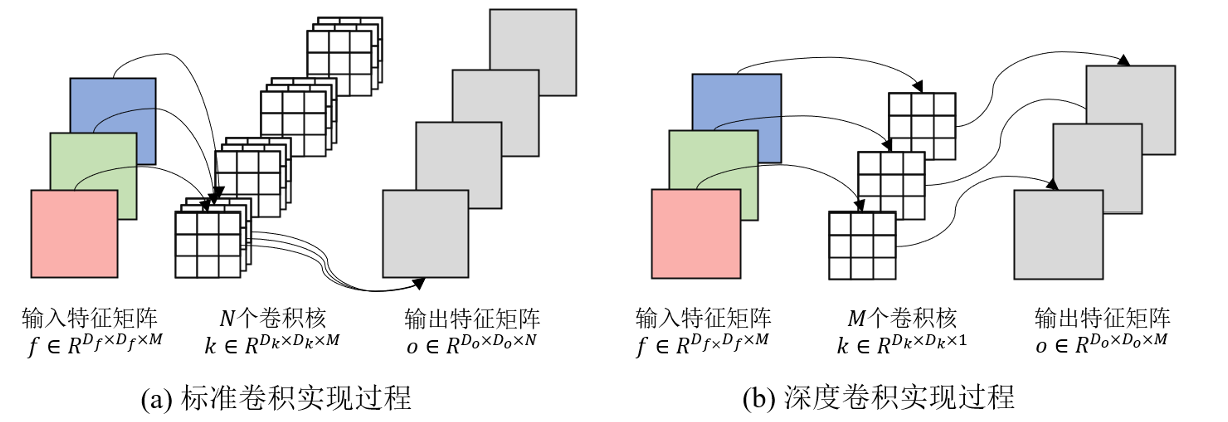
\includegraphics[width=0.8\linewidth]{figures/标准卷积和深度卷积示意图.png}
    \caption{标准卷积与深度卷积示意图}
    \label{fig:dwconv_vs_sconv}
\end{figure}

在深度可分离卷积的支撑下，本文采用倒残差结构作为模块的骨架，以进一步降低信息瓶颈并稳定深层训练。传统残差结构通过恒等映射缓解网络加深带来的梯度消失与性能退化，但当非线性激活作用于低维通道空间时，容易出现信息压缩与细粒度结构丢失。倒残差结构将先压缩后扩张的通道组织方式反转，先通过逐点卷积进行通道扩张，在高维空间内执行非线性变换与空间建模，最后再压缩回原始通道数并与恒等分支相加，从而在保持残差训练稳定性的同时降低低维激活造成的信息损失。倒残差结构如图\ref{fig:inverted_residual}所示。
\begin{figure}[!htbp]
    \centering
    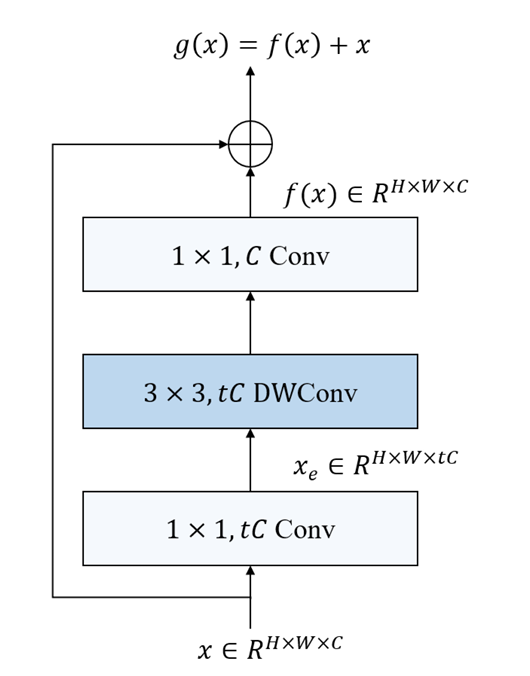
\includegraphics[width=0.5\linewidth]{figures/倒残差结构示意图.png}
    \caption{倒残差结构示意图}
    \label{fig:inverted_residual}
\end{figure}

设输入特征为$X\in\mathbb{R}^{C\times H\times W}$，倒残差框架首先通过通道扩张映射将其升维到$\lambda C$通道，得到
\begin{equation}
X_e=\mathrm{MLP}_e(X)\in\mathbb{R}^{\lambda C\times H\times W},
\label{eq:irmb_expand_new}
\end{equation}
其中$\lambda$为扩张因子。随后在升维空间内引入高效中间算子$\mathcal{F}(\cdot)$进行特征增强，得到
\begin{equation}
X_f=\mathcal{F}(X_e)\in\mathbb{R}^{\lambda C\times H\times W},
\label{eq:irmb_operator_new}
\end{equation}
最后通过通道压缩映射还原通道数，并与恒等分支相加输出
\begin{equation}
Y=X+\mathrm{MLP}_s(X_f), \qquad \mathrm{MLP}_s(X_f)\in\mathbb{R}^{C\times H\times W}.
\label{eq:irmb_residual_new}
\end{equation}
式(\ref{eq:irmb_expand_new})--(\ref{eq:irmb_residual_new})体现了倒残差框架对中间复杂算子计算规模的约束作用，即在保持输入输出维度一致的前提下，将主要计算集中于可控的升维空间，从而在端侧预算内实现更丰富的特征变换。

在高效中间算子 $\mathcal{F}(\cdot)$ 的具体实例化中，标准的多头自注意力机制虽然能够同时学习多组关系建模结果，但在端侧推理中其全量计算会带来较高的矩阵乘法开销。同时在海上雾天场景下，大面积低频散射与背景扰动会使注意力分配趋于平滑，从而弱化对小目标局部高频结构的选择性聚焦。为兼顾全局交互有效性与端侧开销可控性，本文不采用标准多头自注意力作为中间算子，而引入级联分组注意力机制替代其全量注意力计算。两者的关键差异在于信息组织方式：标准多头自注意力将同一输入特征投影到多个子空间并行计算，但各注意力头之间相互独立，最终仅在输出端进行拼接与线性投影；级联分组注意力在构造查询、键、值之前沿通道维将特征显式分组，并通过级联递推将前序分组的输出注入后续分组，使后续分组在关注自身局部子空间的同时继承前序分组的上下文表达，从而在近似预算下提高信息容量并减少冗余计算。级联分组注意力的结构示意如图\ref{fig:cga_arch}所示。
\begin{figure}[!htbp]
    \centering
    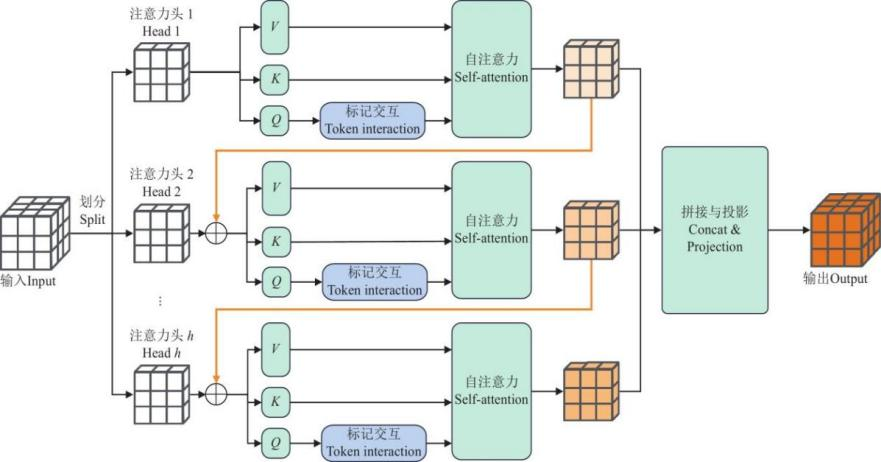
\includegraphics[width=0.9\linewidth]{figures/级联分组注意力模块框架图.png}
    \caption{级联分组注意力模块结构示意图}
    \label{fig:cga_arch}
\end{figure}

设升维特征为$X_e \in \mathbb{R}^{H \times W \times \lambda C}$，沿通道维将其划分为$G$个分组
\begin{equation}
X_e = \mathrm{Concat}\!\left(X_e^{(1)}, X_e^{(2)}, \ldots, X_e^{(G)}\right), \qquad X_e^{(g)} \in \mathbb{R}^{H \times W \times C_g},
\label{eq:cga_split_new}
\end{equation}
其中$\sum_{g=1}^{G}C_g=\lambda C$。为实现组间信息递进，引入级联交互输入$\tilde{X}_e^{(g)}$并定义递推关系
\begin{equation}
\tilde{X}_e^{(1)} = X_e^{(1)}, \qquad
\tilde{X}_e^{(g)} = X_e^{(g)} + \psi\!\left(\tilde{Z}^{(g-1)}\right), \ g \ge 2,
\label{eq:cga_cascade_in_new}
\end{equation}
其中$\tilde{Z}^{(g-1)}$为上一分组的注意力输出，$\psi(\cdot)$为用于维度对齐的线性映射。该递推关系确保第$g$组的注意力计算不仅依赖于自身通道子空间，还显式继承前序分组的上下文表达，从而缓解分组带来的信息割裂并提升特征多样性。在每个分组内部构造查询、键、值线性投影
\begin{equation}
Q^{(g)} = \tilde{X}_e^{(g)}W_Q^{(g)}, \quad
K^{(g)} = \tilde{X}_e^{(g)}W_K^{(g)}, \quad
V^{(g)} = \tilde{X}_e^{(g)}W_V^{(g)},
\label{eq:cga_qkv_new}
\end{equation}
并计算分组自注意力输出
\begin{equation}
Z^{(g)} = \mathrm{Softmax}\!\left(\frac{Q^{(g)}{K^{(g)}}^{\top}}{\sqrt{d_g}}\right)V^{(g)},
\label{eq:cga_attn_new}
\end{equation}
其中$d_g$为该分组的投影维度。最终将各分组输出在通道维拼接并线性映射得到聚合注意力特征
\begin{equation}
Z = \mathrm{Concat}\!\left(Z^{(1)},Z^{(2)},\ldots,Z^{(G)}\right)W_O.
\label{eq:cga_concat_new}
\end{equation}
相较于标准多头自注意力的并行独立头机制，上述级联递推使注意力表达在组间形成渐进式的信息整合，更适合在雾天背景干扰较强时保持对局部结构的选择性，同时避免全量注意力导致的过度平滑。

为兼顾长程交互与局部纹理建模的互补需求，本文将级联分组注意力与深度可分离卷积组合构成倒残差框架内的最终中间算子。记$\mathrm{DWConv}(\cdot)$为$3\times 3$深度可分离卷积，则
\begin{equation}
\mathcal{F}(X_e) = \mathrm{DWConv}(Z) + Z,
\label{eq:cga_dwconv_new}
\end{equation}
其中残差项用于稳定训练并保留注意力输出的主导结构响应。式(\ref{eq:cga_dwconv_new})的组合具有明确的动机：级联分组注意力用于建立跨位置依赖，缓解雾天小目标在深层抽象过程中被大面积海面背景淹没的问题；深度可分离卷积为注意力输出注入局部归纳偏置，使特征在边缘与方向性纹理处保持更高的空间选择性，从而抑制雾天低频散射干扰导致的特征过度平滑。

综上，本文提出的倒残差级联分组自注意力模块以深度可分离卷积降低计算成本，以倒残差升降维框架避免低维非线性带来的信息瓶颈，并以级联分组注意力替代标准多头自注意力以提高雾天场景下全局交互的有效性与选择性。该模块在不显著增加端侧推理负担的前提下强化了微小目标弱响应的上下文可分性，为后续改进残差单元的构建与雾天鲁棒检测性能提升提供了关键的结构支撑。如图\ref{fig:irmb_arch}展示了该模块的具体网络架构。
\begin{figure}[!htbp]
    \centering
    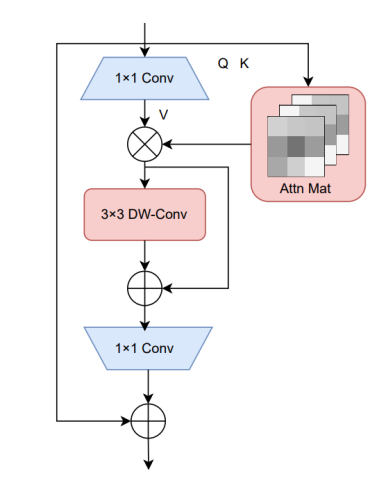
\includegraphics[width=0.5\linewidth]{figures/irmb模块框架图.png}
    \caption{倒残差级联分组自注意力模块结构示意图}
    \label{fig:irmb_arch}
\end{figure}

\subsection{改进残差单元与主干网络}

综合上述针对微小目标弱响应与复杂海面背景强干扰的核心增强机制，本文在标准轻量级残差网络的基础上完成了改进残差单元的构建。无人机嵌入式平台对推理时延与功耗具有严格约束，因此主干网络在设计上必须在特征表达能力与计算复杂度之间取得平衡。本文将无参数三维能量注意力机制与倒残差自注意力模块有序嵌入基本残差单元，旨在不显著增加计算量的前提下，增强浅层结构特征对微弱目标的可分辨性。改进后的整体基本单元结构如图\ref{fig:basicblock_arch}所示。

\begin{figure}[!htbp]
    \centering
    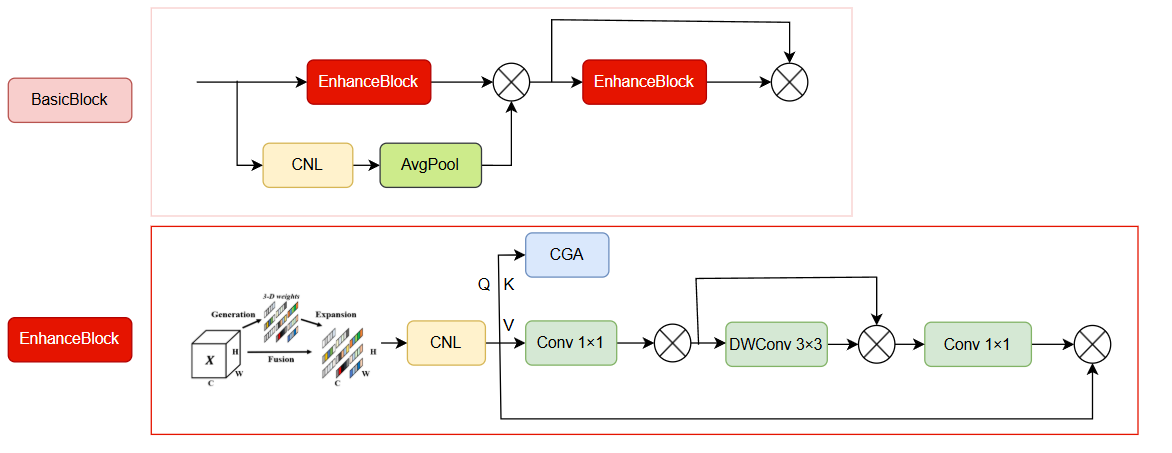
\includegraphics[width=0.8\linewidth]{figures/改进后的basicblock.png}
    \caption{改进后的轻量化残差单元结构图}
    \label{fig:basicblock_arch}
\end{figure}

在卷积特征提取的初始阶段，网络引入无参数三维能量注意力机制对局部响应进行细粒度重标定与背景抑制。对于输入特征张量，该机制基于通道统计量构建能量函数，通过解析解形式为每个神经元生成显著性权重。设单通道特征序列为 $\{x_i\}_{i=1}^{N}$，其能量度量可严密表达为公式\ref{eq:simam_energy_new}。
\begin{equation}
E(x_i) = \frac{(x_i - \mu)^2}{\sigma^2 + \epsilon}
\label{eq:simam_energy_new}
\end{equation}
其中 $\mu$ 与 $\sigma^2$ 分别为该通道特征响应的均值与方差，$\epsilon$ 为防止除零溢出的微小常数。该权重客观反映了神经元相对于背景统计分布的偏离程度，网络据此自适应放大目标区域的微弱高频响应并抑制海面波纹与反射等冗余背景噪声。

经过初步净化的特征随后被送入倒残差级联分组自注意力模块中进行轻量级的长距离空间交互建模，以补充全局上下文语义。该模块的设计思想可归纳为在倒残差结构的通道升降维框架内，嵌入具有动态建模能力的自注意力算子与深度可分离卷积，从而在较低计算成本下扩大有效感受野。最后通过通道压缩映射将特征降维回原始通道数，并与输入形成残差连接。这种混合架构统筹兼顾了卷积神经网络的局部高效性与自注意力机制的全局感知优越性。

改进残差单元的主分支特征处理过程遵循严密的时序逻辑递进。输入特征 $F_{in}$ 首先通过残差主分支的卷积堆叠提取局部结构响应；随后利用三维能量注意力机制进行显著性重标定；紧接着通过倒残差自注意力模块补充上下文语义；最后，该主分支的高阶语义输出与通过跳跃连接直接传递的恒等残差进行逐元素相加，并经过非线性激活函数生成该残差单元的最终输出 $F_{out}$。设标准卷积分支为 $\mathcal{C}(\cdot)$，三维能量注意力机制与倒残差自注意力模块分别记为 $\mathcal{S}(\cdot)$ 与 $\mathcal{R}(\cdot)$，$\delta(\cdot)$ 表示非线性激活函数，则改进残差单元的整体输出映射可严密表达为公式\ref{eq:basicblock_out}。
\begin{equation}
F_{out} = \delta\left(F_{in} + \mathcal{R}\left(\mathcal{S}\left(\mathcal{C}(F_{in})\right)\right)\right)
\label{eq:basicblock_out}
\end{equation}
该组合拓扑结构保留了传统残差网络缓解梯度消失与保障收敛稳定性的优良特性，确保了微小目标特征在逐层前向传递过程中能够得到通道显著性与空间全局性的多维度联合强化。

改进后的轻量级主干网络将持续在三个不同的空间降采样尺度输出特征张量，分别记为集合 $\{C3, C4, C5\}$，供后续的混合编码器与端到端解码器使用。由于本文在整体架构中需要额外引入雾分布表征分支，并在相对高分辨率的 $C3$ 特征节点实施离散小波频域解耦，主干网络浅层细粒度表达的物理真实性与数值稳定性尤为关键。该主干架构为后续的低频散射掩膜分离、环境先验物理特征提取以及多尺度全局交互提供了具备高保真度与强鲁棒性的输入基石。

\section{基于状态空间模型的雾分布表征分支设计}
\label{sec:fog_branch}

第二章的机理分析表明，雾天退化在成像层面体现为透射率衰减与空气光叠加，其统计效应通常表现为低频成分相对增强而高频结构响应被压缩。对于海上无人机航拍任务而言，微小目标的判别信息高度依赖边缘与纹理等结构性响应，当雾气导致局部梯度与高频纹理被弱化时，仅依赖检测主干进行语义抽象将更容易发生目标结构与海面背景扰动的混叠，进而引起漏检与误检。为在保持端到端检测推理流程不变的前提下显式引入雾气空间分布相关的物理先验，本文在检测主干的中间特征层构建雾分布表征分支，分支以形成可被检测网络利用的雾分布表征为核心目标，而非以输出视觉上清晰的图像为最终目标。该分支输出的雾分布先验用于指导检测特征的选择性增强与抑制，使网络能够在特征层面区分受雾严重退化区域与相对可靠区域，从而提升雾天条件下微小目标的可分辨表征。分支结构如图\ref{fig:fog_branch_arch}所示。

\begin{figure}[!htbp]
    \centering
    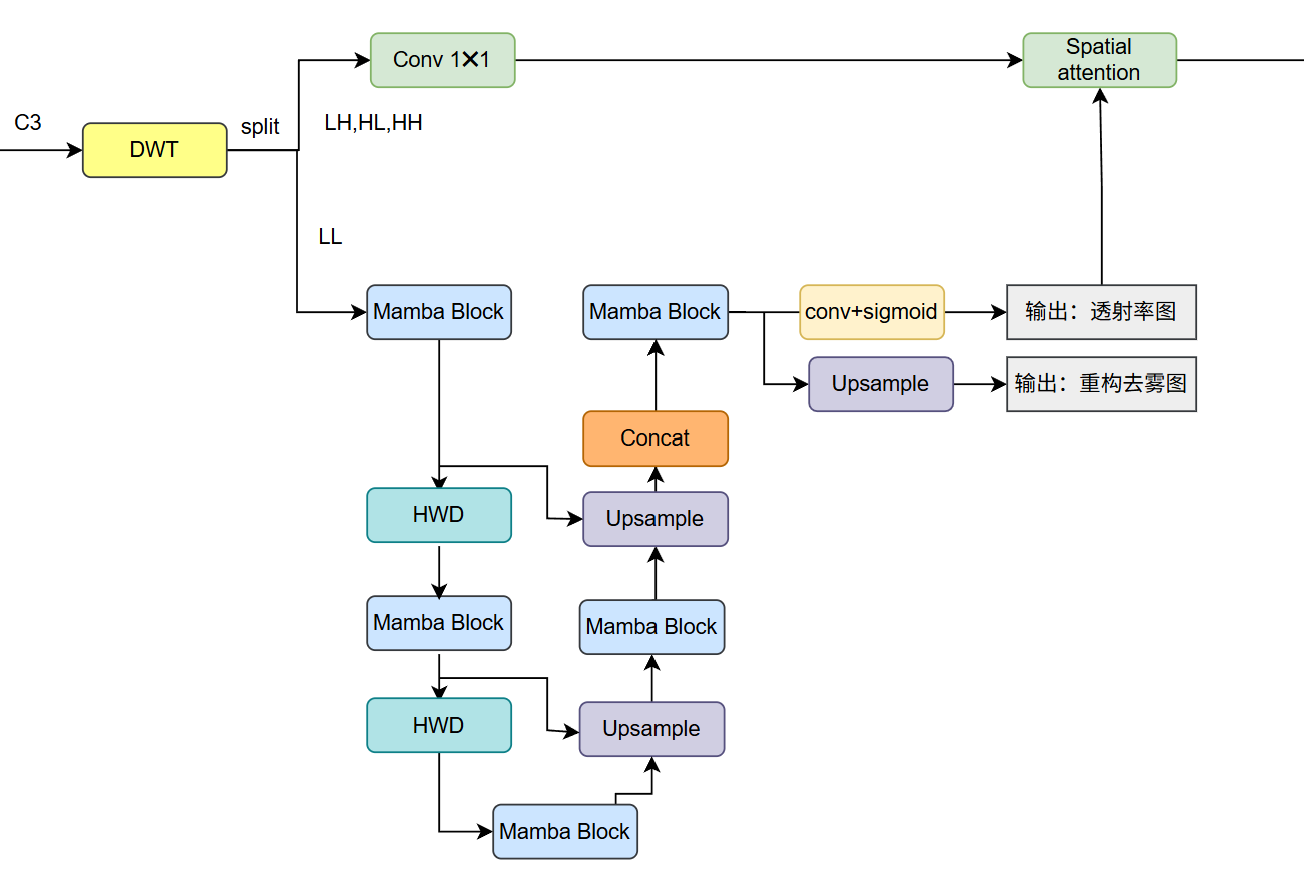
\includegraphics[width=0.85\linewidth]{figures/雾分布表征与特征增强分支结构示意图.png}
    \caption{雾分布表征与特征增强分支结构示意图}
    \label{fig:fog_branch_arch}
\end{figure}

雾气在图像中的空间变化通常呈现平缓连续的分布形态，属于低频主导的背景退化项；与之相对，目标检测所依赖的几何轮廓、边缘梯度与细粒度纹理更集中于高频结构项。若直接在空间域对特征进行增强或重构，容易引入过度平滑并进一步削弱微小目标边缘响应。因此本文首先在检测主干的第三个降采样特征层$C3$处引入离散小波变换以显式分离不同频率子带，将雾分布相关的低频信息与目标结构相关的高频信息解耦，从输入统计上降低高频纹理对雾分布估计的干扰；随后，仅对低频子带构建雾分布表征网络，用以推断与透射率空间变化相关的先验表示；在表征网络内部，为避免标准自注意力在高分辨率特征上出现计算复杂度随序列长度平方增长的问题，并获得对非均匀雾分布的长程依赖建模能力，本文采用状态空间模型，通过线性复杂度的选择性扫描实现全局信息聚合；最后，分支输出雾分布注意图并通过物理引导模块在特征层面对检测主干的语义特征进行调制，实现雾天物理先验与语义信息的协同表达。该设计使雾天鲁棒性提升更多依赖于特征表达与融合机制，而非依赖额外的图像级输出，从而更符合端侧实时约束下的整体优化目标。

设检测主干的输出特征为
\begin{equation}
F_{3}\in\mathbb{R}^{C_{3}\times H_{3}\times W_{3}}.
\end{equation}

为使雾分布估计聚焦于与散射退化相关的低频缓变成分，本文在$C3$特征处引入二维离散小波变换对特征进行频域解耦。离散小波变换通过低通滤波器与高通滤波器在行列两个方向进行滤波与下采样，将输入分解为一个低频近似子带与三个方向性高频细节子带。对单通道二维特征$X\in\mathbb{R}^{H\times W}$，一次分解可写为
\begin{equation}
\mathrm{DWT}(X)\rightarrow \left\{X^{LL},X^{LH},X^{HL},X^{HH}\right\},
\label{eq:dwt_basic2}
\end{equation}
其中$X^{LL}$为低频近似分量，$X^{LH}$、$X^{HL}$与$X^{HH}$分别为水平、垂直与对角方向的高频细节分量。对主干输出特征$F_3$，对各通道进行$\mathrm{DWT}$并在通道维进行组织，得到子带张量$\{F_3^{LL},F_3^{LH},F_3^{HL},F_3^{HH}\}$。一次小波分解后空间尺寸变为$H_3/2$与$W_3/2$，该变换在子带空间内实现了低频与方向性细节的显式分解，为后续低频先验建模与高频细节保留提供入口。

考虑雾分布在统计上更接近低频缓慢变化项，而目标结构更集中于高频细节项，本文仅将$LL$子带作为雾分布表征分支的输入，以降低高频噪声对雾分布估计的干扰，记为
\begin{equation}
F_{low}=F_3^{LL}\in\mathbb{R}^{C_{low}\times \frac{H_3}{2}\times \frac{W_3}{2}}.
\label{eq:fog_ll_input2}
\end{equation}
其余高频子带$\{F_3^{LH},F_3^{HL},F_3^{HH}\}$不进入雾分布表征网络，而在检测流中作为细节旁路保留。为便于与检测主干后续融合，本文将高频子带进行聚合并通过$1\times1$卷积完成通道对齐，记为$\bar{F}_{high}$，其作用是在不引入额外平滑偏置的前提下维持微小目标边缘与纹理信息的可传递性。该频域解耦策略在结构层面形成明确分工，即低频通道用于雾分布先验估计，高频通道保留目标结构细节。


在获得低频子带特征$F_{low}$后，需要构建能够刻画非均匀雾气空间分布的表征网络。若采用纯卷积结构进行估计，模型的有效建模范围仍受限于局部感受野，面对海上雾气跨区域变化明显的情况往往需要堆叠大量卷积层才能覆盖足够大的接收域，从而增加计算成本并削弱端侧部署可行性。标准自注意力虽然具备全局依赖建模能力，但其计算复杂度随空间位置数呈二次增长，对高分辨率特征不具备稳定的计算可扩展性。基于此，本文采用状态空间模型Mamba作为雾分布表征网络的核心算子，以线性复杂度实现长程依赖建模并形成稳定的雾分布表征。

状态空间模型的数学本质是将一维序列建模转化为连续系统的状态更新过程。对于给定的输入序列 $x(t) \in \mathbb{R}$，其连续状态转移偏微分方程可表示为：
\begin{equation}
h'(t) = \mathbf{A}h(t) + \mathbf{B}x(t), \quad y(t) = \mathbf{C}h(t)
\end{equation}
其中 $h(t)$ 为隐状态，$\mathbf{A, B, C}$ 为系统参数矩阵。为使该连续模型适用于深度学习中的离散图像特征，本文引入时间尺度参数 $\Delta$，采用零阶保持器（ZOH）对系统进行离散化逼近，得到离散化参数矩阵 $\bar{\mathbf{A}} = \exp(\Delta \mathbf{A})$ 与 $\bar{\mathbf{B}} = (\Delta \mathbf{A})^{-1}(\exp(\Delta \mathbf{A}) - \mathbf{I}) \cdot \Delta \mathbf{B}$。
将二维低频特征 $F_{low}$ 按照预定扫描顺序展开为离散序列 $x=\{x_n\}_{n=1}^{L}$（$L=\frac{H_3}{2}\cdot\frac{W_3}{2}$），则Mamba模型的核心离散状态更新与输出方程可严密写为：
\begin{equation}
h_{n}=\bar{\mathbf{A}} h_{n-1}+\bar{\mathbf{B}} x_{n},\qquad y_{n}=\mathbf{C} h_{n}
\end{equation}
区别于常规SSM，本文引入了选择性扫描机制（Selective Scan），使得参数 $\bar{\mathbf{B}}, \mathbf{C}, \Delta$ 成为依赖于输入 $x_n$ 的动态函数。这种输入感知机制使得模型能够在雾气浓度突变的区域自适应地调整特征的遗忘与保留权重，以线性复杂度实现对长程依赖的建模能力，更适合刻画非均匀雾分布的跨区域连续性。

状态空间模型的基本思想是将序列建模转化为状态更新过程。对于输入序列 $\{x_t\}$，状态空间模型可写为
\begin{equation}
h_{t+1} = A(x_t)h_t + B(x_t)x_t,
\end{equation}

\begin{equation}
y_t = C(x_t)h_t,
\end{equation}
其中 $h_t$ 为隐状态，$y_t$ 为输出，$A(\cdot),B(\cdot),C(\cdot)$ 为输入相关参数映射。Mamba引入选择性扫描机制，使状态更新能够根据输入内容动态调整特征保留与遗忘强度，从而提高对不同区域退化差异的表征能力。在二维特征上，本文采用二维选择性扫描结构对 $F_{low}$ 进行多方向序列化扫描，使其能够捕获水平与垂直方向的长距离相关性，适应雾气在图像平面上的连续分布特征。在雾分布表征分支结构设计上，本文采用多层Mamba块堆叠，并在分支内部引入上采样与跨层连接以保持较高空间分辨率。该设计的关键目标是避免通过多次下采样导致的空间信息压缩，因为透射率先验需要在较细粒度空间尺度上提供可靠的区域划分。该分支在输出端通过通道压缩映射得到环境先验特征 $P$，并进一步生成透射率注意力图 $T$：
\begin{equation}
T = \sigma(W_t * P),
\end{equation}
其中 $W_t$ 为 $1\times1$ 卷积核，$\sigma(\cdot)$ 为Sigmoid激活函数，$T\in[0,1]^{1\times H'\times W'}$ 表示空间透射率权重。$T$ 的数值越大表示区域信息相对可靠，越小表示退化更强。该注意力图在后续章节中作为物理引导信息参与检测特征重标定。

将二维特征$F_{low}$按照预定扫描顺序展开为序列$u=\{u_n\}_{n=1}^{L}$，其中$L=\frac{H_3}{2}\cdot\frac{W_3}{2}$。状态空间模型的离散状态更新与输出方程可写为
\begin{equation}
s_{n}=A s_{n-1}+B u_{n},\qquad
y_{n}=C s_{n}+D u_{n},
\label{eq:ssm_state2}
\end{equation}
其中$s_n$为隐状态，$y_n$为输出，$A,B,C,D$为可学习参数矩阵。为使表征网络能够根据输入内容自适应选择性地保留或抑制信息，本文采用输入相关的门控调制对状态更新过程进行动态控制，使模型在雾分布变化显著区域保留更多有效信息，在平坦区域抑制冗余传播。该选择性机制与线性复杂度的状态更新共同保证了模型对大范围非均匀雾分布的全局刻画能力与端侧计算可控性。

在实现层面，状态空间块对序列输出$y$进行重排以恢复空间结构，得到二维特征$Y\in\mathbb{R}^{C_{ssm}\times \frac{H_3}{2}\times \frac{W_3}{2}}$。随后通过轻量卷积投影与归一化映射生成雾分布表征特征$P$，并进一步压缩到可作为空间调制权重的注意图$T$：
\begin{equation}
T=\sigma\!\left(\mathrm{Conv}_{1\times 1}(P)\right),
\label{eq:fog_T2}
\end{equation}
其中$\sigma(\cdot)$为Sigmoid函数，$T\in[0,1]^{1\times \frac{H_3}{2}\times \frac{W_3}{2}}$用于表征不同空间位置的雾分布强弱程度并作为后续物理引导融合的核心介质。需要强调的是，式(\ref{eq:fog_T2})中的$T$在本文中作为雾分布表征的归一化表示，其物理解释是对空间可靠性的量化提示，用于指导检测特征的选择性增强与抑制，而非作为图像级复原的最终输出。

在雾分布表征分支中，状态空间模型由低频子带生成雾分布注意图$T\in\mathbb{R}^{1\times H_T\times W_T}$，其物理含义可解释为不同空间位置的退化程度或可靠性指示。与此同时，检测主干在$C3$节点经离散小波变换得到的高频细节子带$\{LH,HL,HH\}$携带微小目标的边缘与纹理结构信息。为了在不引入额外图像级输出的条件下，将低频雾分布先验有效注入高频结构特征并服务于后续检测，本文在$C3$分支位置构建通道选择性物理引导融合模块。该模块以雾分布注意图为显式先验，在空间维与通道维两个层面完成对高频特征的自适应调制，从而实现对雾天退化区域的选择性补偿以及对可靠结构响应的稳定保留。

设$C3$雾分布表征分支经通道映射后得到高频特征$F_H\in\mathbb{R}^{C\times H\times W}$，其中通道映射由逐点卷积实现，用于对齐后续颈部特征的通道维度。由于$T$由低频路径生成，其空间分辨率与$F_H$可能不一致，首先通过可微尺度对齐算子$\Psi(\cdot)$将$T$重采样到与$F_H$一致的尺寸，得到
\begin{equation}
T_s=\Psi(T;H,W),\qquad T_s\in\mathbb{R}^{1\times H\times W}.
\label{eq:pgm_align_c3}
\end{equation}
在空间调制阶段，本文采用残差式增益调制以避免直接乘法抑制导致微小目标响应进一步衰减。具体地，定义空间调制后的高频特征为
\begin{equation}
\tilde{F}_H = F_H + \alpha \left(F_H \odot T_s\right),
\label{eq:pgm_spatial_residual}
\end{equation}
其中$\odot$表示逐元素乘法并在通道维广播，$\alpha$为可学习缩放系数。式(\ref{eq:pgm_spatial_residual})保留了恒等通路，使得当$T_s$在局部存在估计偏差时不会引发特征分布的灾难性偏移，同时在雾天退化显著区域能够对结构响应提供增益补偿。

仅以空间权重调制仍难以刻画不同语义通道对雾气退化的敏感性差异。雾天条件下，部分通道更易受到低频散射背景与海面反光的干扰而产生冗余激活，而与微小目标几何结构相关的通道则更需要被强调。为此，本文在空间调制之后引入通道重标定机制，在通道层面对$\tilde{F}_H$进行选择性加权。首先对$\tilde{F}_H$执行全局平均池化获得通道描述向量
\begin{equation}
z=\mathrm{GAP}(\tilde{F}_H)\in\mathbb{R}^{C},
\label{eq:pgm_gap}
\end{equation}
其中$\mathrm{GAP}(\cdot)$表示在空间维$(H,W)$上的均值聚合。随后采用轻量两层感知机生成通道权重向量
\begin{equation}
w=\sigma\!\left(W_2\,\delta\!\left(W_1 z\right)\right)\in\mathbb{R}^{C},
\label{eq:pgm_se}
\end{equation}
其中$W_1\in\mathbb{R}^{\frac{C}{r}\times C}$与$W_2\in\mathbb{R}^{C\times\frac{C}{r}}$为可学习参数矩阵，$r$为通道压缩比，$\delta(\cdot)$为非线性激活函数，$\sigma(\cdot)$为Sigmoid函数。最终输出的通道选择性引导特征定义为
\begin{equation}
\hat{F}_H = w \odot \tilde{F}_H,
\label{eq:pgm_channel_out}
\end{equation}
其中$w$在空间维进行广播以匹配$\tilde{F}_H$的张量尺寸。式(\ref{eq:pgm_channel_out})使网络能够在不显著增加推理开销的前提下抑制更易受雾干扰的冗余通道响应，并突出对微小目标判别更关键的结构性通道表征。

上述空间调制与通道重标定共同构成$C3$节点处的通道选择性物理引导融合过程。该过程以低频路径输出的雾分布注意图为显式物理先验，对高频细节特征进行结构保持型增强，并将增强后的$\hat{F}_H$回注入后续颈部特征融合链路。由此，雾分布先验在特征层面实现对高频结构响应的自适应加权，引导检测主干在雾天条件下获得更稳定的微小目标结构表征与更高的目标-背景可分性。

为保证雾分布注意图$T$具有稳定的物理一致性并避免在联合训练早期退化为无意义响应，本文在雾分布表征网络末端引入双路输出拓扑。第一路输出为雾分布注意图生成分支，通过$1\times1$卷积与Sigmoid产生$T$，作为检测特征调制的核心介质。第二路输出为重构监督分支，其目的在于提供强约束信号，促使状态空间表征确实学习到与散射退化一致的低频先验，而非仅拟合检测损失的短期梯度噪声。该重构分支由上采样与卷积映射组成，将低频先验特征映射回图像空间并输出重构图$I_{rec}$，在训练阶段与清晰标签$I_{gt}$计算像素级一致性损失：
\begin{equation}
\mathcal{L}_{rec}=\left\|I_{rec}-I_{gt}\right\|_{1}.
\label{eq:rec_loss2}
\end{equation}
式(\ref{eq:rec_loss2})的作用在于约束增强分支在低频先验空间中学习与大气散射退化相一致的映射关系，从而提升$T$的可解释性与稳定性。推理阶段仅保留雾分布注意图$T$用于特征调制，并移除重构监督支路以避免额外计算开销对实时性造成影响。该训练与推理的分离策略使分支在训练阶段获得稳定的物理先验表征能力，在推理阶段以轻量方式输出空间先验用于检测特征重标定。

\section{分阶段协同训练策略设计}
\label{sec:training_strategy}

在本文提出的雾天小目标检测框架中，主干检测路径与环境增强路径共同参与特征形成与判别映射。两条路径在功能目标上存在显著差异，检测路径的优化目标是类别判别与边界框回归，其监督信号来自实例级人工标注，而环境增强路径的核心作用是学习雾气退化的空间分布规律并输出可用于调制检测特征的先验信息，其表征质量高度依赖于对物理退化过程的稳定拟合。若在联合训练初期即对两条路径同时施加强耦合的检测损失监督，雾分布表征分支在尚未形成有效物理先验表征时会受到庞大检测梯度的强烈牵引，导致其输出的透射率注意力掩膜趋于退化为无判别性的常数分布，进而削弱物理引导融合机制的实际作用。与此同时，端到端检测任务的稀疏一对一匹配监督在海上小目标密集场景下极易导致正样本数量严重不足，使得训练早期解码器收敛极其缓慢，从而进一步加剧了联合优化过程中的梯度震荡与次优收敛风险。基于上述多任务优化固有的梯度冲突与匹配缺陷，本文设计了分阶段协同训练策略，通过先验能力独立预热、检测阶段解耦微调与辅助监督增强三项连贯机制，从工程底层保障整体模型在恶劣雾天场景下的稳定收敛与感知性能提升。

本文将整体联合训练过程划分为先验预热阶段与检测协同阶段。先验预热阶段的核心目标是使雾分布表征分支在特征域内纯粹地学习到与雾天退化物理规律相一致的映射关系，使其最终输出的透射率注意力图具有严密的空间可解释性与数值稳定性。该阶段仅激活雾分布表征分支的低频先验建模链路，并在分支尾端临时接入重构监督头以形成可独立优化的目标。网络输入为雾天退化图像，雾分布表征分支输出透射率相关物理特征并通过重构支路生成去雾重构图像。为保证重构监督对结构细节不过度强调从而引入不必要的平滑偏置，本文采用绝对误差损失作为核心监督项。该损失函数对局部异常值具有极强的鲁棒性质，能够在一定程度上抑制雾天数据中局部高光反射区域对网络梯度的绝对主导作用，促使雾分布表征分支更稳定地学习全局低频物理退化规律。重构监督的根本目的并非追求人类视觉感官上最优的图像复原质量，而是通过对齐清晰无雾标签来强行约束环境雾分布表征分支的特征隐空间，使其生成的透射率注意力掩膜与真实雾气退化强弱保持高度一致。在具体的数据流向控制上，此预热阶段彻底阻断了物理引导特征融合模块以及检测主干深层解码器的前向传播，不执行任何多尺度检测损失计算，从而在大幅降低训练初期显存占用与计算负担的同时，彻底杜绝了检测梯度对物理先验学习的早期破坏。

进入检测协同阶段后，网络全面加载预热阶段获得的稳定环境雾分布表征分支权重，并正式接入随机初始化的动态物理引导特征融合模块与完整的端到端检测链路。此阶段的核心技术难点在于保证脆弱的物理先验表征在激烈的检测微调过程中不发生灾难性语义漂移，从而避免透射率注意力掩膜退化为无效的冗余权重。为此本文采用了严密的参数梯度截断与流向拦截策略。具体而言，雾分布表征分支中用于生成透射率特征的核心参数在检测协同阶段被完全冻结，其仅作为离线的物理特征提取器供融合模块实时调用，同时预热阶段专用的上采样重构头在此阶段被彻底移除，不再参与任何前向预测与反向传播。设雾分布表征分支参数集合为 $\Theta_{\text{enc}}$，检测及融合相关参数集合为 $\Theta_{\text{det}}$，在检测阶段对 $\Theta_{\text{enc}}$ 实施严格的梯度截断，即强制约束 $\nabla_{\Theta_{\text{enc}}}\mathcal{L} = 0$，检测相关参数的更新严格遵循公式\ref{eq:gradient_update}所示的迭代准则，其中 $\eta$ 为优化学习率，$t$ 为训练迭代步数。该解耦优化策略显著降低了多任务联合训练的优化不确定性，使新接入的物理引导融合模块能够在绝对稳定可靠的环境先验条件下，专心学习最高效的跨域特征重标定方式。在端到端检测损失的具体形式上，本文沿用集合预测范式，检测总损失由焦点分类损失、交并比损失以及几何一致性回归约束项加权构成，在匈牙利二分图匹配算法的严格约束下实现预测框与真实目标的一一对应。
\begin{equation}
\Theta_{\text{det}}^{(t+1)} = \Theta_{\text{det}}^{(t)} - \eta \nabla_{\Theta_{\text{det}}}\mathcal{L}_{\text{det}}
\label{eq:gradient_update}
\end{equation}

常规的端到端检测解码器高度依赖于上述的一对一匹配监督机制，但这种极度稀疏的监督信号在处理海上微小目标密集场景时暴露出了严重的收敛瓶颈。一对一匹配导致每张图像中能够被划分为正样本的预测框数量极其有限，训练早期的解码器难以获取足够的有效梯度，极易在复杂的雾天退化背景下产生定位漂移与漏检。为从根本上提高训练阶段的监督密度，本文在检测协同阶段引入协作混合分配监督机制，在主干混合编码器输出的增强特征序列上并行附加多个辅助检测头。这些辅助预测头采用经典的一对多密集标签分配策略来生成更为丰富的正负样本对，从而大幅增强对骨干网络的梯度反馈并显著提升微小目标的特征学习效率。设混合编码器输出特征为 $F_{enc}$，附加的辅助检测头集合为 $\{\mathcal{H}_k\}_{k=1}^{K}$，则第 $k$ 个辅助头的前向输出为 $\hat{Y}_k = \mathcal{H}_k(F_{enc})$。训练阶段的全局总损失可严密拓展为公式\ref{eq:total_hybrid_loss}所示。
\begin{equation}
\mathcal{L} = \mathcal{L}_{\text{det}} + \sum_{k=1}^{K}\gamma_k \mathcal{L}_k
\label{eq:total_hybrid_loss}
\end{equation}
其中 $\mathcal{L}_{\text{det}}$ 为主解码器的一对一集合预测损失，$\gamma_k$ 为设定的辅助损失平衡权重，$\mathcal{L}_k$ 则为第 $k$ 个辅助头在一对多分配策略下独立计算的分类与边界框回归联合损失。该协作混合结构通过多头密集监督迫使编码器输出具备更强语义判别性的鲁棒特征，并为主解码器提供了更为精准的先验锚点指导。在模型最终的推理部署阶段，所有基于一对多分配的辅助检测头均被彻底剥离，网络仅保留单一的主解码器进行高效的集合预测，从而在不增加任何额外端侧推理算力成本的前提下，完美实现了检测精度的零成本跃升。

为确保上述分阶段协同训练策略在实际实验环境中的严格可复现性与极致性能释放，本文详细明确了训练过程中的核心工程超参数配置。在先验预热阶段，网络使用AdamW优化器进行参数更新，初始学习率设定为千分之一，并配合余弦退火策略进行平滑衰减，预热总周期设定为五十个全局迭代轮次，以确保雾分布表征分支能够充分拟合合成雾天数据集的物理散射规律。进入检测协同阶段后，网络加载预热参数并切换至多尺度联合微调模式，检测主干与物理融合模块的初始学习率保守调整为万分之一，以避免过大的参数更新步长破坏已有的稳定特征空间分布。此外，协作混合分配监督中的辅助损失平衡权重 $\gamma_k$ 在训练初期设定为一以提供强烈的密集梯度引导，而在微调的最后二十个迭代轮次中，采用线性衰减策略将其逐步降至零，促使网络在收敛末期彻底向主解码器的一对一精确匹配范式过渡。上述详尽的工程约束方案在优化目标上实现了显式的阶段分解，在梯度传播路径上实现了物理级别的严格解耦，为复杂环境感知模型在小样本雾天数据条件下的稳定收敛提供了极其扎实的工程可行性保障。

本文将训练过程划分为先验预热阶段与检测协同阶段。先验预热阶段的目标是使雾分布表征分支在特征域内学习到与雾天退化规律一致的映射关系，使其输出的透射率注意力图具有空间可解释性与稳定性。检测协同阶段在加载预热权重的基础上，将先验输出用于检测特征调制，并在保持先验表征稳定的条件下优化检测损失，使检测头与融合模块能够充分利用环境先验信息完成鲁棒预测。

在整体损失构造上，先验预热阶段的优化目标可表示为
\begin{equation}
\min_{\Theta_{\text{enc}}}\ \mathcal{L}_{\text{rec}}(I_{rec}, I_{gt}),
\end{equation}
其中 $\Theta_{\text{enc}}$ 表示雾分布表征分支相关参数集合，$I_{rec}$ 为重构输出，$I_{gt}$ 为清晰监督图像，$\mathcal{L}_{\text{rec}}$ 采用像素级一致性损失以约束先验学习的物理一致性。检测协同阶段的优化目标为
\begin{equation}
\min_{\Theta_{\text{det}}}\ \mathcal{L}_{\text{det}}(\hat{Y},Y),
\end{equation}
其中 $\Theta_{\text{det}}$ 表示检测相关参数集合，包含主干检测路径、动态物理融合模块、编码器与解码器参数，$\mathcal{L}_{\text{det}}$ 为端到端检测损失。两阶段训练在参数更新层面形成明确分工，避免在优化早期出现多任务梯度相互干扰导致的先验失效或检测不稳定。

先验预热阶段仅激活雾分布表征分支的低频先验建模链路，并在分支尾端临时接入重构监督头以形成可优化目标。该阶段输入为雾天退化图像 $I_{fog}$，环境增强分支输出透射率相关特征 $P$ 并通过重构支路生成去雾重构图像 $I_{rec}$。为保证重构监督对结构细节不过度强调从而引入平滑偏置，本文采用 $L_1$ 损失作为主要监督项：
\begin{equation}
\mathcal{L}_{\text{rec}} = \|I_{rec}-I_{gt}\|_1.
\end{equation}
该损失具有对异常值更鲁棒的性质，能够在一定程度上抑制雾天数据中局部高光区域对梯度的主导作用，使雾分布表征分支更稳定地学习全局低频退化规律。重构监督的作用并非追求视觉质量最优，而是通过对齐清晰标签约束雾分布表征分支的特征空间，使其生成的透射率注意力 $T$ 与雾气退化强弱保持一致，从而为后续检测阶段提供可用先验。

在实现层面，预热阶段仅保留雾分布表征分支与重构头的前向计算，不执行检测解码器与多尺度检测损失计算，从而降低训练初期的显存占用与计算负担，并减少检测梯度对先验学习的干扰。该阶段完成后保存雾分布表征分支参数，作为检测协同阶段的初始化权重。

在检测协同阶段，网络加载预热得到的雾分布表征分支权重，接入动态物理引导融合模块与完整检测链路。此阶段的关键在于保证先验表征在训练过程中不发生灾难性漂移，从而避免透射率注意力退化为无效权重。为此，本文采用冻结与拦截策略：雾分布表征分支用于生成 $T$ 与 $P$ 的核心参数在检测协同阶段保持冻结，仅作为前向先验供融合模块调用；预热阶段用于重构监督的上采样重构头在检测阶段被移除或拦截，不参与前向与反向传播。该处理使检测损失的梯度主要作用于检测路径与融合模块参数，从而将优化过程聚焦于如何使用先验提升检测性能，而非迫使雾分布表征分支适配检测损失。

设雾分布表征分支参数为 $\Theta_{\text{enc}}$，检测相关参数为 $\Theta_{\text{det}}$，则检测阶段的参数更新满足
\begin{equation}
\Theta_{\text{enc}} \leftarrow \Theta_{\text{enc}}, \quad \Theta_{\text{det}} \leftarrow \Theta_{\text{det}} - \eta \nabla_{\Theta_{\text{det}}}\mathcal{L}_{\text{det}},
\end{equation}
其中 $\eta$ 为学习率。该解耦优化策略显著降低了联合训练的不确定性，使融合模块能够在稳定先验条件下学习更有效的特征重标定方式。

在检测损失形式上，本文沿用端到端集合预测范式的损失构造，检测损失由分类损失与边界框回归损失构成：
\begin{equation}
\mathcal{L}_{\text{det}} = \mathcal{L}_{\text{cls}} + \lambda_1 \mathcal{L}_{\text{l1}} + \lambda_2 \mathcal{L}_{\text{giou}},
\end{equation}
其中 $\mathcal{L}_{\text{cls}}$ 为分类损失，$\mathcal{L}_{\text{l1}}$ 为边界框回归损失，$\mathcal{L}_{\text{giou}}$ 为几何一致性约束项，$\lambda_1,\lambda_2$ 为权重系数。该损失在匈牙利匹配约束下实现预测集合与真实目标集合的一一对应，从而避免非极大值抑制等后处理对推理速度造成的影响。


端到端检测解码器通常采用一对一匹配监督，监督信号相对稀疏。对于海上小目标密集场景，一对一匹配导致的正样本数量有限，训练早期解码器收敛较慢，容易在雾天退化背景下产生定位漂移。为提高训练阶段的监督密度，本文在检测协同阶段引入协作混合分配监督机制，在编码器输出特征上附加多个辅助检测头，通过一对多标签分配生成更丰富的正样本对，从而增强梯度反馈并提升小目标学习效率。

设编码器输出特征为 $F_{enc}$，附加的辅助检测头集合为 $\{\mathcal{H}_k\}_{k=1}^{K}$，则第 $k$ 个辅助头输出为
\begin{equation}
\hat{Y}_k = \mathcal{H}_k(F_{enc}).
\end{equation}
辅助头采用密集分配策略生成正样本集合，并计算对应的辅助损失 $\mathcal{L}_k$。训练阶段总损失可写为
\begin{equation}
\mathcal{L} = \mathcal{L}_{\text{det}} + \sum_{k=1}^{K}\gamma_k \mathcal{L}_k,
\end{equation}
其中 $\gamma_k$ 为辅助损失权重。该结构通过多头监督使编码器输出具备更强判别性，并为解码器提供更充分的正查询指导，有助于改善雾天条件下小目标的定位稳定性。推理阶段仅保留主解码器输出，所有辅助头被移除，因此不会增加部署时的计算成本。

综合上述设计，本文训练流程遵循先预热后协同的两阶段范式。预热阶段以重构监督约束雾分布表征分支学习稳定的低频先验映射，检测协同阶段冻结雾分布表征分支并优化检测路径与融合模块，辅以辅助检测头增强监督密度。该流程在优化目标上实现显式分解，在梯度传播路径上实现解耦控制，使先验表征能够在训练全程保持有效，从而保证物理引导融合机制在雾天场景下产生可量化的检测性能增益。

本节提出的分阶段协同训练策略为后续实验章节的对比与消融提供可操作的训练范式，同时也为复杂结构在小样本雾天数据条件下的稳定收敛提供工程可行性保证。
\section{本章小结}
\label{sec:chap3_summary}

本章围绕海上雾天无人机航拍小目标检测任务在退化条件下易出现特征弱化与语义混淆的问题，给出了面向雾天场景的轻量级端到端检测模型设计，并对核心结构与训练策略进行了系统阐述。本章在所选端到端目标检测框架基础上，针对雾天小目标易退化、特征表达不足等问题进行了系统性的结构优化。首先论述了引入倒残差模块与三维注意力机制改进轻量化主干网络的设计方案，显著提升了微小目标特征的表达能力。其次深入剖析了基于状态空间模型的雾分布表征分支，阐明了利用离散小波变换分离高低频特征以实现雾天细节信息有效恢复的理论机制。随后推导了动态物理引导特征融合机制，通过通道自适应对齐与注意力重标定加强了环境先验与语义信息的协同表达，并阐述了级联分组机制在多尺度交互中的优化作用。最后提出了包含参数预热、特征冻结拦截以及添加辅助多重分配检测头在内的分阶段协同训练策略，从工程优化层面保障了联合模型的稳定收敛与整体性能提升。本章的整体模型架构设计与底层机制推导，为后续开展定量的实验验证与检测性能客观评估确立了完整且严密的方法基础。

